\section{Modellierung von Regelstrecken}
\subsection{Bsp. Vorwärtsbewegung beim Auto \formelbuch{57}}
\begin{minipage}[]{8cm}
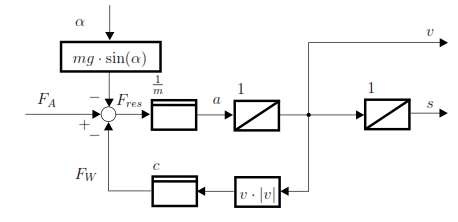
\includegraphics[width=8 cm]{./bilder/auto.png}
\end{minipage}
\hspace{1cm}
\begin{minipage}[]{10cm}
Resultierende Kraft $F_{Res}$: Neben der Kraft des Antriebs $F_A$ spielen der Luftwiderstand $F_W$ und die durch die Neigung der Strasse verursachte Kraft $F_S$ eine Rolle: $F_{Res}(t) = F_A(t) - F_W(t) - F_S(t)$\\\\
Luftwiderstand $F_W$: Der Luftwiderstand wächst quadratisch mit der Geschwindigkeit v [m/s]: $F_W = c \cdot v(t)^2 \cdot  sign(v(t)) = c \cdot v(t)\mid v(t)\mid$\\\\
Kraft $F_S$ durch Strassenneigung: 
$F_S(t) = mg \cdot sin(\alpha(t))$\\\\
Beschleunigung a: Die Beschleunigung a ist gegeben durch: $a(t) = \frac{F_{Res(t)}}{m}$
\end{minipage}

\subsection{Stationäre Signale}
	Für den stationären Fall gelten folgende Bedingungen:
	\begin{itemize}
    	\item \textbf{Integratoren} haben am \textbf{Eingang Null}.
    	\item \textbf{Integratoren} haben am \textbf{Ausgang} einen \textbf{beliebigen Wert}.
    	\item \textbf{Totzeitglieder} werden kurzgeschlossen.
    	\item \textbf{PT$_1$-Glieder} wirken als \textbf{P-Glieder} mit $K_P = K_{PT_1}$ behandelt.
    	\item (\textbf{Fehlersignale} werden jeweils als \textbf{Null} angenommen.) \textbf{Mit Vorsicht annehmen}
  	\end{itemize}
  	\newpage